% Created 2018-09-16 Son 02:31
% Intended LaTeX compiler: pdflatex
\documentclass[a4paper,twoside]{article}
\usepackage[utf8]{inputenc}
\usepackage[T1]{fontenc}
\usepackage{graphicx}
\usepackage{grffile}
\usepackage{longtable}
\usepackage{wrapfig}
\usepackage{rotating}
\usepackage[normalem]{ulem}
\usepackage{amsmath}
\usepackage{textcomp}
\usepackage{amssymb}
\usepackage{capt-of}
\usepackage{hyperref}
\usepackage[T1]{fontenc}
\usepackage{lmodern}
\usepackage[margin=3.5cm]{geometry}
\usepackage{pdflscape}
\author{David Pham}
\date{\today}
\title{Multivariate Time Series Classification and Embedding}
\hypersetup{
 pdfauthor={David Pham},
 pdftitle={Multivariate Time Series Classification and Embedding},
 pdfkeywords={},
 pdfsubject={},
 pdfcreator={Emacs 25.2.1 (Org mode 9.1.7)}, 
 pdflang={English}}
\begin{document}

\maketitle
\tableofcontents


\section{Project overview}
\label{sec:org59cffe4}

In the financial investment industry, the speed and the quality of processing
information is what determines if a business is successful or failure. In the
recent period, an emphasis has been set on machine learning algorithms for
investment strategies. One common application is the statement of the algorithms
to perform classification of companies to put them into sector.

This project aims to create and review algorithms for classifying companies by
using their share price. We will test a heuristic classifier using sample
correlation and train a deep neural network to mimic the performance the sample
correlation and study the hidden layer of the network. The projects uses data
from Quandl and SimFin.

Time series modeling using deep learning in a financial context has been studied
by \href{https://journals.plos.org/plosone/article?id=10.1371/journal.pone.0180944\#sec009}{Bao and Yue (2017)}, where share prices are predicted using a combination of
wavelet transform, autoencoders and long-short term memory units. \href{https://arxiv.org/pdf/1802.03628.pdf}{Qiu et al.
(2018)} studies how to create fast inference of correlation of between time
series by applying discrete Fourier transform and uses the frequency domain of
the time series as embedding for the input. A dense neural network is then
trained to create a model that predict correlations between embedding of the
time series. Several loss function are studied and lead to different embedding.
Our work differs as our methods keeps in time domain of the time series and aims
to classify them more as to find the nearest neighbors and to predict them
accurately and efficiently. Additional reference can be found in the
aforementioned papers.

\section{Problem Statement}
\label{sec:org46a4ecf}

The goal of this project is to create a method to embed financial time series
into a vector space and analyze qualitatively the embedding. The main
challenge to complete this projects are following.

\begin{enumerate}
\item Filter the universe of the data and acquire the data from different
sources.
\item Transform data to be usable in machine learning algorithm.
\item Create artificial data to transform the problem into a supervised learning problem.
\item Create a base model and train an advanced classifier to create the embedding.
\item Analyze briefly the embedding.
\end{enumerate}




\section{Metrics}
\label{sec:orgda57672}

We will use the \emph{accuracy} defined as the ratio between the true positive and
negatives predictions divided by the dataset size. Or in formula

\begin{align*}
  \textrm{accuracy} = \frac{\textsc{number of correct classification} }{\textsc{sample size}}
\end{align*}

This metric is relevant because at a certain level the algorithms should be
able to assign correctly the stock price of companies to the sector of the
companies.

Compared to other metrics, the accuracy targets our ability to predict the
sector of each companies. As our model aims to be as general as possible,
there is no particular additional cost of having false negative or false
positive, hence the accuracy is a suitable metric for metric.


\section{Data}
\label{sec:orge8906e6}

The below table shows the data and how to access them.

\begin{center}
\begin{tabular}{lllr}
Type & Provider & Access to Datatest & Downloaded\\
\hline
Price & \href{https://www.quandl.com/databases/WIKIP/documentation/about}{Quandl} & \href{https://www.quandl.com/databases/WIKIP}{Quandl API} & 2018-08-21\\
Company information & \href{https://simfin.com/data/find/}{SimFin} & \href{https://s3.us-east-2.amazonaws.com/udacity-capstone-data-davidpham87/data/company\_fundamentals.csv}{S3} & 2018-08-21\\
Stocks Returns & Processed & \href{https://s3.us-east-2.amazonaws.com/udacity-capstone-data-davidpham87/data/wiki\_stocks\_returns.csv}{S3} & 2018-09-11\\
Index Returns & Processed & \href{https://s3.us-east-2.amazonaws.com/udacity-capstone-data-davidpham87/data/wiki\_indices\_returns.csv}{S3} & 2018-09-11\\
\hline
\end{tabular}
\end{center}

In our analysis, we used the closed price of the US companies provided by
Wikipedia and distributed by Quandl. As we additionally required the sectors
from the company we needed to merge it with an additional databases provided by
SimFin, which provides the taxonomy created by Global Industry Classification
Standard (GICS). We could find the sectors of \emph{726} companies which
constituted our dataset. The prices range from 1962 to 2018.

The stocks returns have a mean 7 basis points (0.0007) and median of 0, whereas
the standard deviation is at 10 percent. When the returns are bounded between
the 5th and 95th quantile, they range between -3.6\% and 3.8\% which are loosely
normally distributed with a standard deviation estimated at 1.5\%. The returns
display some maximum values that are abnormal (like a share price multiplication
by 99, which can be possible but are exceptional).

Concerning the indices returns, by construction their min and max values are set
to -10\% and 10\%. When filtering the indices returns lying between the 5th and
95th quantile, they range between -2.1\% and 2.2\% and seems to follow a Gaussian
distribution with mean 0 and standard deviation of 1.5\%.

\section{Exploratory Analysis}
\label{sec:org89bc8d0}

In Figure \ref{fig:distribution-sectors} and \ref{fig:gics-level}, one can
observe that number of stocks per sectors and the synthetic indices created by
aggregating the returns.

We observe that financial services, technology and oil and gas are the most
prominent sectors. At first glance, the indices seems to be behave according to
our intuition to the economic situation from the last decades. We see clear two
downward pikes which coincide with the bubble dot-com and the financial crisis.

\begin{figure}    
\begin{center}
  \label{fig:distribution-sectors}
  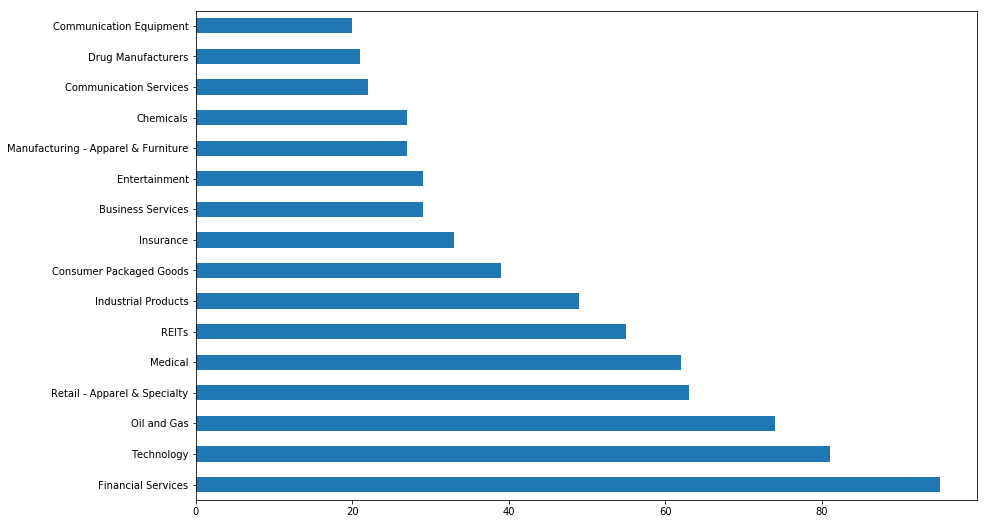
\includegraphics[width=0.95\textwidth]{figures/sectors_distribution}
  \caption{Distribution of sectors in the data.}
  \end{center}
\end{figure}

\begin{figure}    
\begin{center}
  \label{fig:gics-level}
  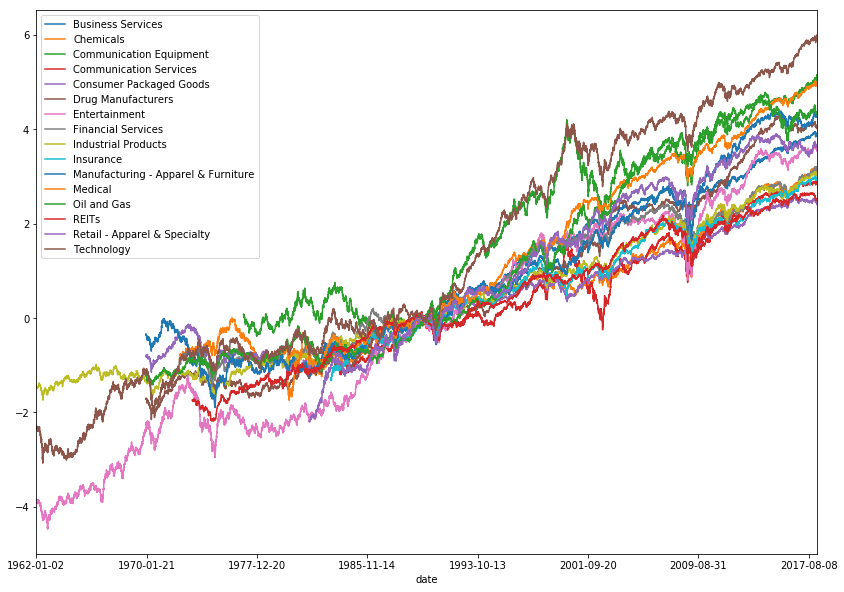
\includegraphics[width=0.95\textwidth]{figures/indexes_level}
  \caption{Synthetic indices of sectors according to GICS. Index are set on 100 on the 1990-01-01.}
  \end{center}
\end{figure}

\section{Algorithms and Technique}
\label{sec:org90358cc}

There is two classifiers. One is algorithmic and the is other one is based on
a dense neural network using the right transformation of the input to
incorporate non linear relationship between the weights.

The first classifier computes correlations of time-series and then assign to an
input time-series the \emph{sector} with which it has the highest correlation. 

For two random variables \(X\) and \(Y\), with sufficient stability assumption, the
Pearson correlation is defined as

\begin{align*}
  \rho_p(X, Y) = E[XY] - (E[X]E[Y])^2 \approx \sum_{i=1}^n x_iy_i - \Big(\sum_{i=1}^nx_i\sum_{i=1}^n y_i\Big)^2,
\end{align*}

This first rule based method does not require any parameter fitting (which
makes it appealing with some respect). 

The second classifier use a deep neural network to create features and
representation (or state) of the inputs to be able to separate linearly all
the output sectors (or classes). 

A deep neural network can be understood as a powerful mapping \(f_\theta\)
between the input and the output. In our particular case, \(f_\theta\) can be
interpreted as function composition of many simpler models whose output have
been transformed by a non-linear function (called activation function). The
goal of these composition is to support the network to design by himself
relevant transformations of the input, called embedding or latent variables,
to help it improving its predictions.

The challenge of the designer of the network is to specify the type and size
of these inner simpler function and the non linear function linking them to
create a model whose input transformations will generalize to out of sample
data.

The model then predicts its output by using these transformations of the input
spaces by creating partition of the space. A good intuition of the last step
can gain on \href{https://playground.tensorflow.org}{Playground Tensorflow}.

Another challenge is to be able to find optimal weights \(\hat\theta\) for
\(f_\theta\). This problem is solved by running optimization algorithms trying
to reduce a loss function. The choice of the loss function and the
optimization algorithm are key decision for the training of the model.

We use the \emph{categorical cross entropy} loss in our model, which basically
minimize the probability of the model to pick the wrong sector. We train the
neural network using \emph{Adam}, which optimize the parameters of the network by
minimizing the loss using stochastic gradient descent algorithm which
standardizes the gradient and also updates it in iteration. In detail, it
means that our optimizer creates estimates of \(\theta\) and update \(\theta\) of
\(f_\theta\) in the direction such that the loss diminishes the most. The size
of the update is named the learning rate. The direction, also called the
gradient, is estimated on a sample of observations, the so-called batch, and
\emph{Adam} creates a weighted average the latest estimator of the gradient and the
new (standardized) estimator. This method allows to have more stability of the
gradient between batches and ease the training of the network. The batch size
was set to 128, the learning rate starts at \(0.001\) with a learning rate
scheduler that diminish the learning by tenfold if the metrics has not been
improved in the last 10 epoch.

Additionally, dropout functions, functions that mask the output of previous
layers were incorporated into our neural network to support it to avoid
over-fitting.

Concerning the input of the model, the data was split into training, dev, and
test set using with 80\%, 10\%, 10\% of the overall data set. In the training
phase, each instance of a batch we sampled randomly a companies of the training
set, sampled a 3 months (63 days) of observation of the companies' stock
returns along with the returns of the sector indices.

\section{Benchmark}
\label{sec:org9548d7c}

Intuitively, we could use random guessing as a benchmark (this would yield a
13\% accuracy at best as Financial Services is the biggest represented class).
A bit more challenging, we could use correlation as measure of association and
using the sector with the highest correlation to our input series, This
classifier gets an accuracy rates of 59\%.


\section{Methodology}
\label{sec:orgdf4002a}

\subsection{Data processing}
\label{sec:orge16cd46}

From the Quandl dataset, the prepossessing involves keeping only the ticker
and the close price for as many date as possible and as many companies as
possible. Then the table is joined to the SimFin dataset containing sectors
for 726 companies. In total we have 16 sectors, from which we can extract
data. Due to the lack of GICS sectors, a few sectors were merged together to
increase their size, e.g. all the Oil and Gas companies were merged into a
single sector.

Then the sector indices were created by averaging the daily returns of the
stocks within the sectors. The returns were floor and capped to 10\% as it is
unlikely that a indices of stocks lose or gain more than 5\% in a single
trading day and the 100 level was set for 1990-01-01.

\subsection{Implementation}
\label{sec:org6549843}

The integrity of the code follows a linear process in the \texttt{notebook} folder
of the project. One should be able to run all the code in each notebook
separately. It was considered to have a proper implementation in the project
and to avoid code duplication, but under time constraint, copy paste solution
were preferred. That being said, the code has been written using pure python
functions to avoid spaghetti code.

The implementation using Tensorflow and the keras API linked in the library.
The Keras API allowed to defined our network and our model into a simple
function and wrap customized transformation into the \texttt{keras.Lambda} layer.
The exact implementation can be found in the notebooks. We launched AWS
server with spot instance and launched a jupyter server there and made it
accessible to our web-browser. We develop code also in the terminal with
Emacs to adapt some code.

The first step was to download the data from the several providers and to
process them as discussed in the previous section. Namely, we need to
construct \texttt{pandas} dataframe (modeled as data frame with time index) of
returns of stocks and synchronize theses returns with the returns of the
sectors. We decided to simply create a single big data frame with repeated
values as the size of our data could largely be hold in memory.

The model is fed with 63 days of observations of stocks returns with sector
returns in order predict one of 17 classes. The implementation of the model
is defined through \texttt{keras} layers and custom functions. One particular custom
function is to multiply the standardize returns of the stock with the sectors
returns date by date to create the non-linear features. Keras function
(models) only accept in a tensor/array format, hence the previous data frame
need to be transformed into numpy array. In practice, we engineer three
manual features to the model, the multiplication of the returns date by date,
the sign of the previous operation and independent monthly correlation. These
engineered features are then feed to different fully connected layers with
relu activation, their results are concatenated and fed to a dense layer
which creates the embedding, from which a last layer will create a partition
for the classification. 

In order to speed up the training phase, we needed to use several classes
from keras to support asynchronous loading of the data thanks to the
\texttt{Sequence} object. During training, batches were creating by sampling 128
sectors uniformly with resampling and select a random company (with uniform
probability) in the selected sectors, this insure the classes are balanced as
some sectors contains more stocks and ease the training.

As a technical detail, whenever the analysis and the training of the model
occur in different scripts, the label encoder from scikit which maps the
sectors into number should be at best serialized or insure its inputs are
similar between the running time. Otherwise, there is a significant risk that
the label encoder swap classes and destroy the perform of the classifier.


\section{Refinement}
\label{sec:org73b2063}

The implementation has been performed with a simple function defining the
network. We ran several experiment of the network, using convolutional
networks, with adaptation of inception units and residual units, known in the
neural network for images, but they did not lead to any improvement of the
model. Moreover, to avoid overfitting, we added several batch normalization
layers as well as Gaussian noise layer with a really small standard deviation.
A few layers in the network were penalized \(L_2\) regularization to insure that
the features stayed as independent as possible.

The best models were the ones which were fed with correlations and forwarded
to into a dense networks. The reason is associative measure a non linear and
it is not common to multiply inputs with each other. That being said, we
managed to create a convolutional layer that achieved an accuracy rate of
55\%, a bit short from our best model and from the benchmark, but using only
linear transformation.


\subsection{Structure of the network}
\label{sec:orgf675192}

The network is depicted in Figure \ref{fig:keras-nn}. From the input data,
three transformation are performed. The first one create product of
normalized observation in order to let the model to detect smaller pattern of
interaction. The second transformation performs the same computation but on
the sign of the input. This should create a more robust estimate of measure
of association. The third is to compute the correlation matrix as feature for
the model. We concatenate them and create a dense layer for creating the
embedding from which we extract the classes.


\begin{figure}    
\begin{center}
  \label{fig:keras-nn}
  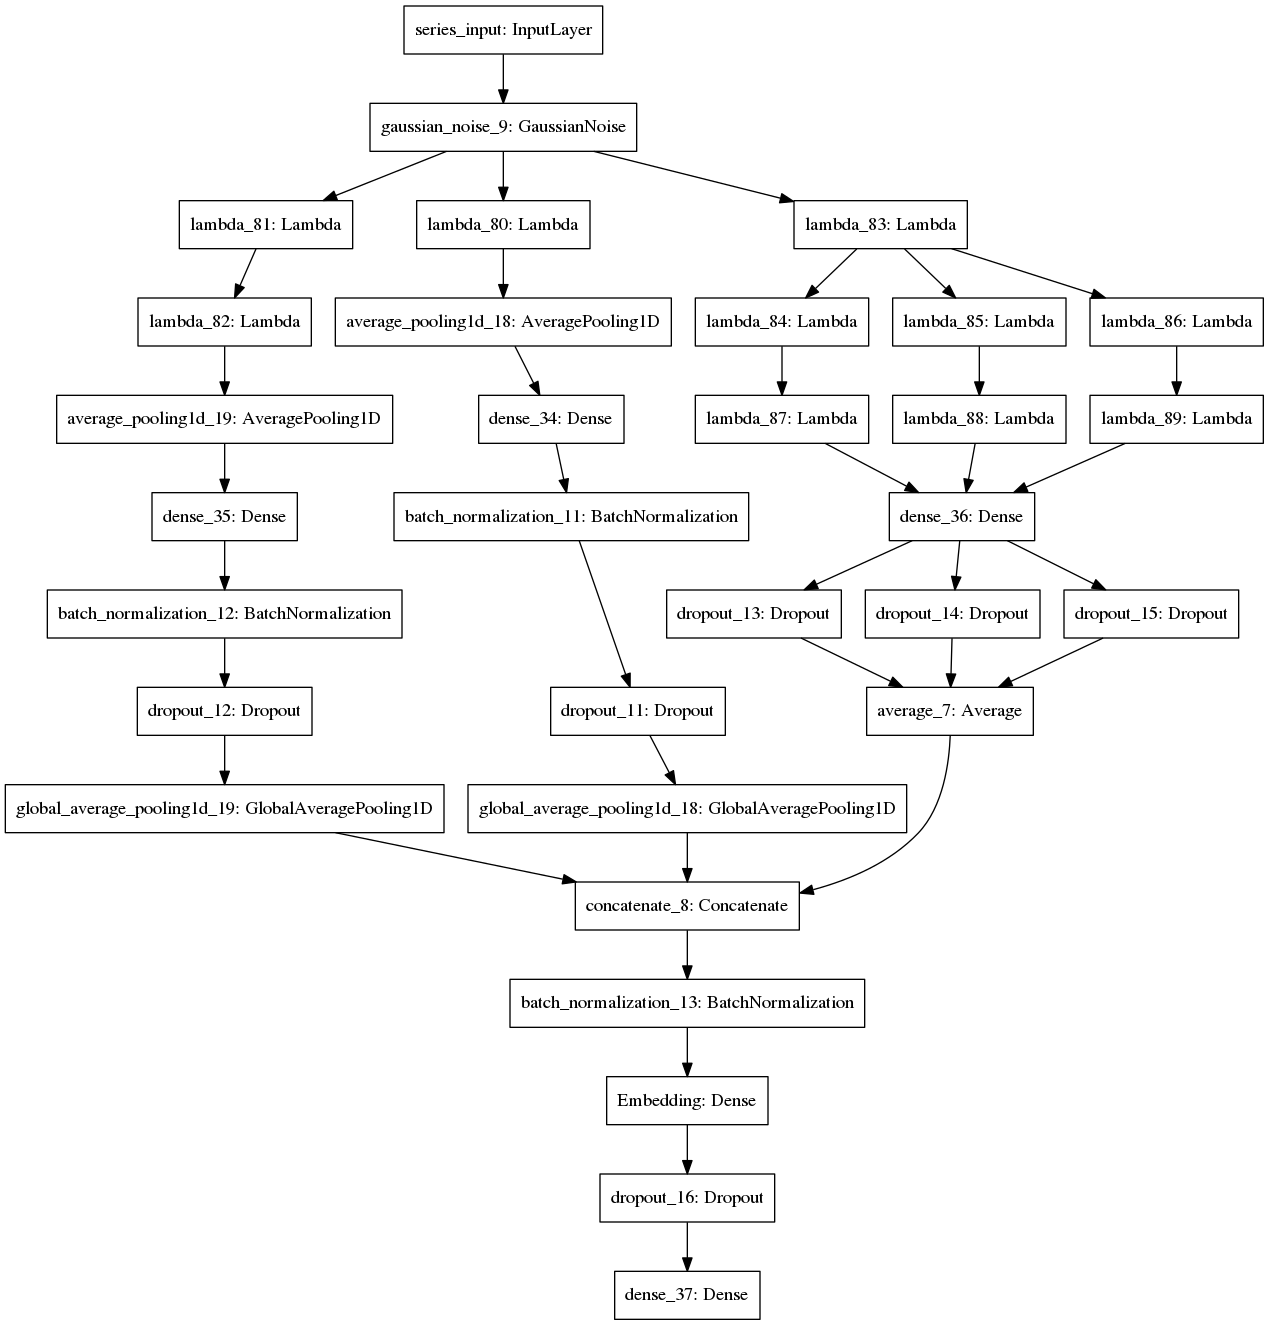
\includegraphics[width=\textwidth]{./figures/model_keras}
  \caption{Neural Network structure}
  \end{center}
\end{figure}


\section{Results}
\label{sec:orgd2caaf1}

The base model using only correlation for the period of 3 months achieves
\(59%\) accuracy in training and test set. This rather rule based method is
really good.

As for neural network model, it achieves around \(58\%\) percent accuracy on a
single observation of three months which is on par with our benchmark.
However, when we provide 25 random samples of 3 months period to the
classifier, the classifier achieves \(80\%\) accuracy. As it can be read in
Table \ref{tab:org9c87c36}

\begin{landscape}
  \begin{figure}    
  \begin{center}
    \label{fig:confusion-matrix}
    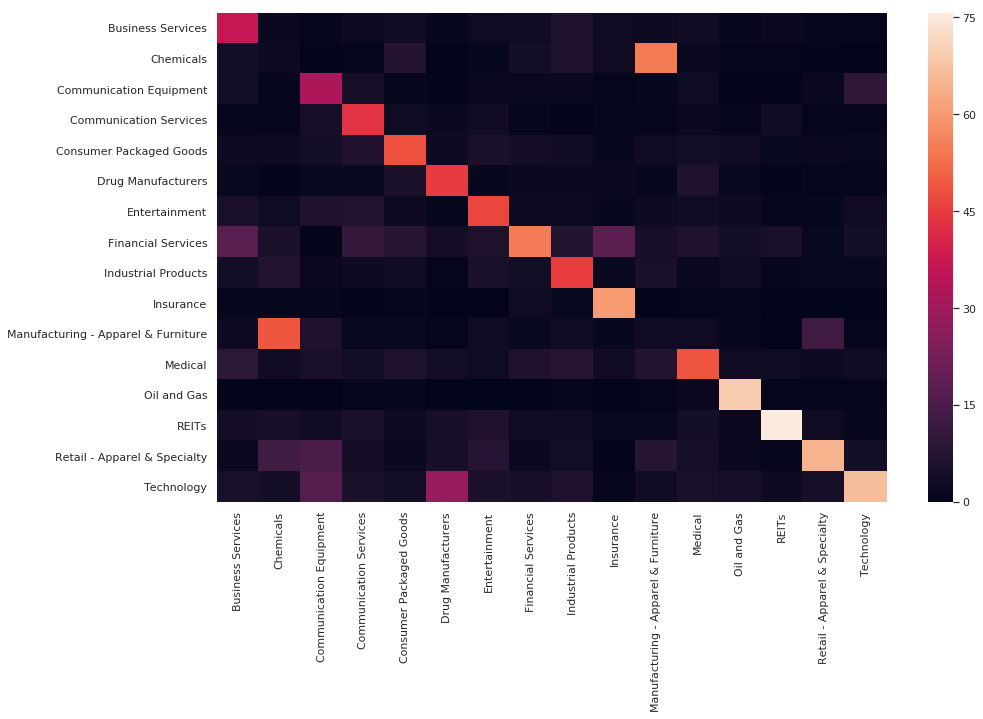
\includegraphics[height=\textheight]{./figures/confusion_matrix.png}
    \caption{Confusion matrix of our predictor.}
    \end{center}
  \end{figure}
\end{landscape}

In Figure \ref{fig:confusion-matrix}, we observe that the neural network model
classifier does a fairly good job at classifying sectors with a notable
exception of \emph{Chemicals} and \emph{Manufacturing - Apparels and Furniture}. The
reason are probably that are little data.

The model is robust to input data as the input is standardized in the first
step of the model and even a non-parametric feature (which is invariant to
scale) is used in our model. As our training method heavily relies on sampling
time period, stocks and dropout nodes, the optimal model is stable with
respect to the random seed.

The model's performance generalize well to unseen stocks as the numbers in the
in Table \ref{tab:org9c87c36} and \ref{tab:org57ac37e} corroborate.
These Tables displays the performance of the classifier to unseen companies
over different periods of time. Table \ref{tab:org57ac37e} shows the
performance of the classifier when it predicts the class of a company by
aggregating the prediction over 25 sample periods.


\begin{longtable}{|l|rrrr|}
\caption{\label{tab:org9c87c36}
Confusion Report from the neural network classifier with 21 days observation data of companies from the test set.}
\\
\hline
 & precision & recall & f1-score & support\\
\hline
\endfirsthead
\multicolumn{5}{l}{Continued from previous page} \\
\hline

 & precision & recall & f1-score & support \\

\hline
\endhead
\hline\multicolumn{5}{r}{Continued on next page} \\
\endfoot
\endlastfoot
\hline
Business Services & 0.74 & 0.26 & 0.39 & 4474\\
Chemicals & 0.63 & 0.55 & 0.59 & 2662\\
Communication Equipment & 0.41 & 0.52 & 0.46 & 926\\
Communication Services & 0.52 & 0.44 & 0.47 & 2307\\
Consumer Packaged Goods & 0.59 & 0.51 & 0.54 & 3715\\
Drug Manufacturers & 0.47 & 0.31 & 0.37 & 1603\\
Entertainment & 0.56 & 0.56 & 0.56 & 2344\\
Financial Services & 0.68 & 0.69 & 0.69 & 9241\\
Industrial Products & 0.46 & 0.49 & 0.48 & 4091\\
Insurance & 0.59 & 0.34 & 0.43 & 2807\\
Manufacturing - Apparel \& Furniture & 0.80 & 0.49 & 0.61 & 2031\\
Medical & 0.48 & 0.67 & 0.56 & 8339\\
Oil and Gas & 0.80 & 0.62 & 0.70 & 8897\\
REITs & 0.75 & 0.69 & 0.72 & 5815\\
Retail - Apparel \& Specialty & 0.42 & 0.63 & 0.50 & 5740\\
Technology & 0.57 & 0.60 & 0.59 & 8122\\
Utilities & 0.64 & 0.95 & 0.77 & 3686\\
\hline
avg / total & 0.61 & 0.59 & 0.59 & 76800\\
\hline
\end{longtable}

\begin{longtable}{|l|rrrr|}
\caption{\label{tab:org57ac37e}
Confusion Report from the neural network classifier with resampled data of 21 days from companies from the test set.}
\\
\hline
 & precision & recall & f1-score & support\\
\hline
\endfirsthead
\multicolumn{5}{l}{Continued from previous page} \\
\hline

 & precision & recall & f1-score & support \\

\hline
\endhead
\hline\multicolumn{5}{r}{Continued on next page} \\
\endfoot
\endlastfoot
\hline
Business Services & 1.00 & 0.67 & 0.80 & 3\\
Chemicals & 1.00 & 1.00 & 1.00 & 3\\
Communication Equipment & 1.00 & 1.00 & 1.00 & 2\\
Communication Services & 1.00 & 0.50 & 0.67 & 2\\
Consumer Packaged Goods & 1.00 & 1.00 & 1.00 & 4\\
Drug Manufacturers & 0.00 & 0.00 & 0.00 & 2\\
Entertainment & 1.00 & 1.00 & 1.00 & 3\\
Financial Services & 1.00 & 1.00 & 1.00 & 10\\
Industrial Products & 1.00 & 1.00 & 1.00 & 5\\
Insurance & 1.00 & 1.00 & 1.00 & 3\\
Manufacturing - Apparel \& Furniture & 1.00 & 1.00 & 1.00 & 3\\
Medical & 0.67 & 1.00 & 0.80 & 6\\
Oil and Gas & 1.00 & 1.00 & 1.00 & 7\\
REITs & 1.00 & 1.00 & 1.00 & 6\\
Retail - Apparel \& Specialty & 1.00 & 0.83 & 0.91 & 6\\
Technology & 0.80 & 1.00 & 0.89 & 8\\
Utilities & 1.00 & 1.00 & 1.00 & 4\\
\hline
avg / total & 0.93 & 0.94 & 0.92 & 77\\
\hline
\end{longtable}


\subsection{Benchmark comparison}
\label{sec:org45ebadd}

As mentioned previously, the model with no opinion (or constant answer) has
an accuracy of at best 12\% (the proportion of financial companies). Using the
rule based method of choosing the class with the highest correlation, the
model would yield an accuracy of around 59\%. In light of these number, our
classifier for a single period is slightly better (2\% better accuracy) versus
the rule based method, but it has the advantage of yielding embedding and
also incorporate several measure of dependency. Moreover, it has the
possibility to incorporate additional dependence measure that just the
highest correlation.

\section{Embedding}
\label{sec:org6a416c4}

We are curious to look at the embedding produce by our neural network. We use
t-SEN to create a low dimensional representation of it. This technique
preserves the similarity between points.

In order to create an estimate of the embedding, we sampled the 25 periods of
3 months of each stock and averaged their embedding. 

In Figure \ref{fig:tine-embedding}, it can be observed that stocks from the
same sector tends to be near each other. The distinct cluster are finance and
technology, which are also the most represented in our dataset. The model
seems to have difficulty to differentiate some chemical companies as their
embedding seems to be close to some industrial production companies. In
general, the more companies we had in the raw dataset the more precise the
groups are.

\begin{landscape}
  \begin{figure}    
  \begin{center}
    \label{fig:tine-embedding}
    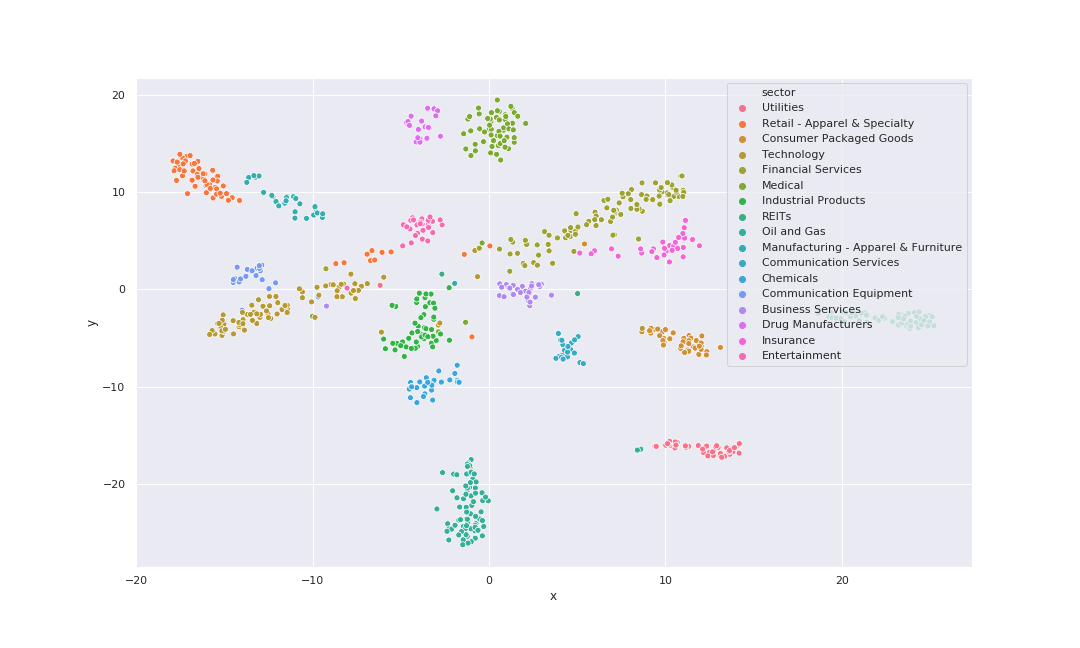
\includegraphics[height=\textheight]{./figures/tsne.png}
    \caption{T-SNE of the embedding layers of the network.}
    \end{center}
  \end{figure}

  \begin{figure}    
  \begin{center}
    \label{fig:silhouette-score}
    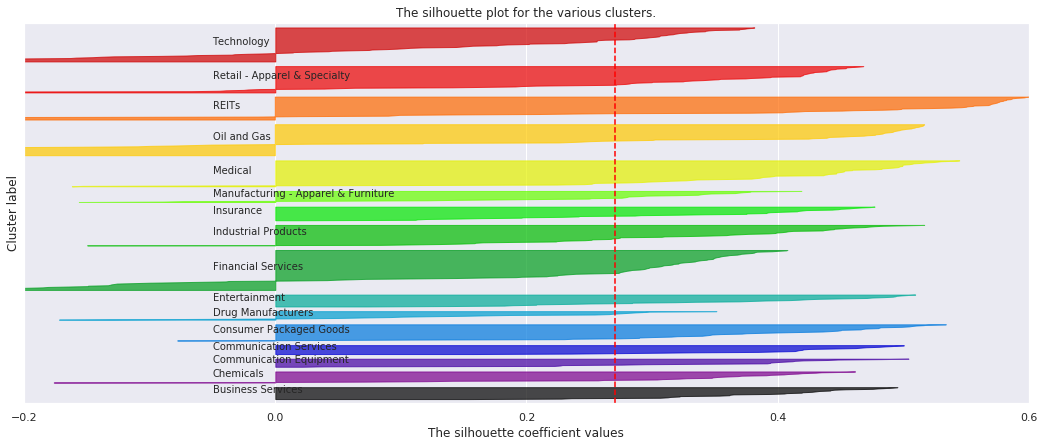
\includegraphics[height=\textheight]{./figures/silouhette_score}
    \caption{Silhouette score of the average embedding of the stocks}
    \end{center}
  \end{figure}
\end{landscape}

In Figure \ref{fig:silhouette-score}, the silhouette score is depicted for the
several sectors in our dataset. The first observation is we see the advantage
of a neural network classifier over k-means clustering, because the silhouette
score over-weights the mislabeled sample of financial and technology, which are
the most precise sectors. Otherwise we can observe that REiTS, Oil and Gas,
and the Insurance sector are grouped tightly making them quite distinct group.


\section{Conclusion and Further applications}
\label{sec:org8bd0427}

The first lesson I learned is data preparation and acquisition is much harder
than thought and we should thank the machine learning community for providing
so many labeled data set for our development. Indeed the financial industry
still leverage on providing exclusive data and create a difficult task to
leverage on alternative dataset, which could potentially provide added value.

Second, in deep learning, a bigger network does not necessarily translate into
a better performance: training is much more difficult with more parameters
even with regularizers and advanced optimization method. As for the training,
balancing the classes improves a lot the training and can potentially improve
the performance of the model. Financial data also proved to be tricky to
handle without proper averaging. The signal to noise ratio is much higher than
typical machine learning application domain.

The primary goal of the project was to find method that could create embedding
for financial time series and Figure \ref{fig:tsne-embedding} provides a good
proof that this goal has been reached. Our clustering abilities are still
lacking as the accuracy rate for sample of three months is yet not better than
a simple correlation measure. But the method has a higher accuracy when
sampled with more data. 

As for the improvement, we could try different architecture (LSTM and several
skip convolution). The LSTM models could allow flexible time input. Moreover
it would have been interesting to apply some semi-unsupervised method to
improve the model and embedding. We could have applied our existing predictor
for stocks whose sector is missing and recompute the indices and maybe retrain
the classifier. A really interesting step would have been to incorporate T-SNE
or \href{https://github.com/lmcinnes/umap}{Uniform Manifold Approximation and Projection} in the training and apply
additional clustering technique. These low dimensional projections seems to
cluster data efficiently. This could also potentially resolve our inability to
detect new group in as we would need to train them. Zero shot learning would
be an interesting project to the study.
\end{document}